\normalsize
\subsection*{Schwarz Method}
\begin{figure}[htbp]
  \begin{center}
    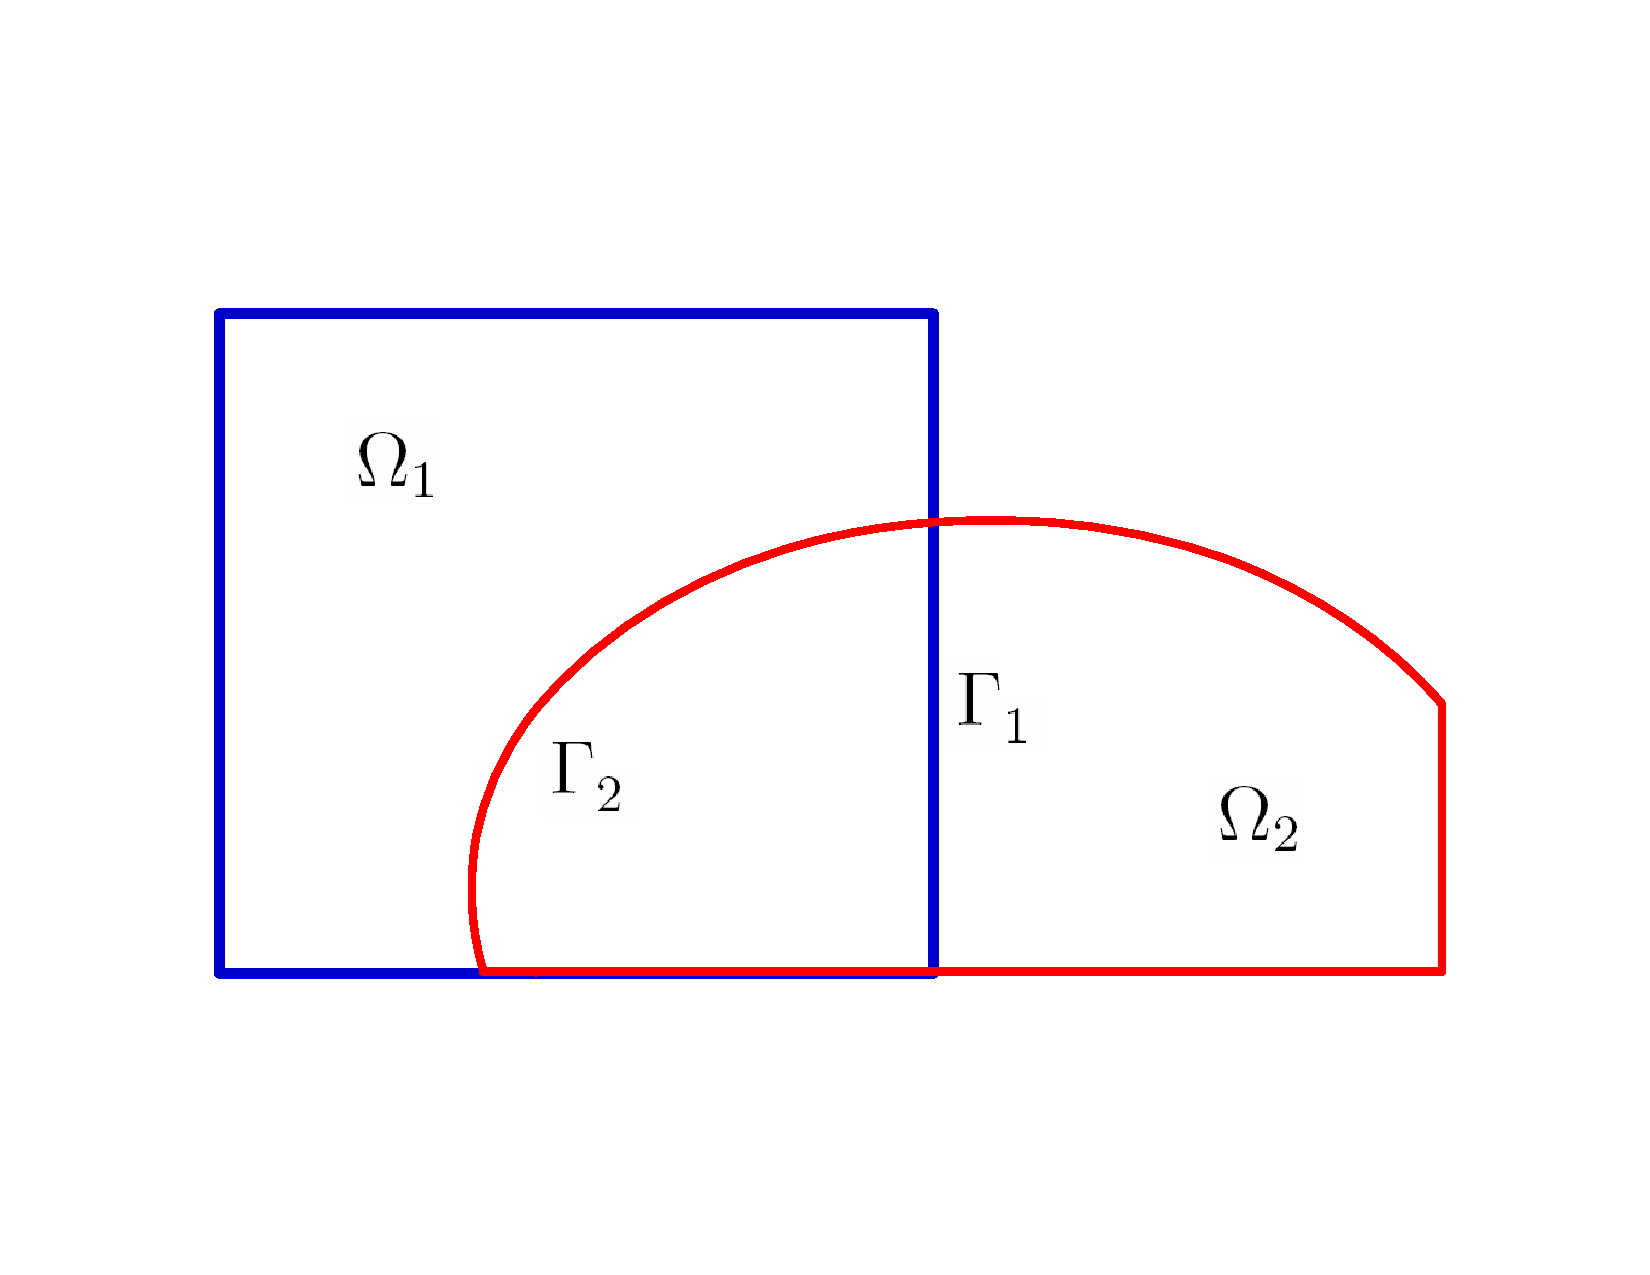
\includegraphics[scale=0.3]{../figures/Schwarz.pdf}
    \caption{Overlapping Schwarz Method.}
    \label{fig:Schwarz}
  \end{center}
\end{figure}
The Schwarz alternating method \cite{Schwarz1869} can be used to decompose the solution domain of iterative solvers for the Poisson equation. For a simplified two-subdomain case, the partial differential equation is first solved in subdomain $\Omega_1$ with Dirichlet boundary condition on the boundary $\Gamma_1$,
\be
\left\{
\baa{ccccc}
A_{1}\phi_1^n & = & B_1   & in & \Omega_1 \\
\phi_1^n    & = & \phi_2^{n-1}|_{\Gamma_1} & on & \Gamma_1
\eaa
\right.
\label{eqn:Schwarz-multi-1}
\ee %u_1^n    & = & g     & in & \p \Omega_1 \backslash \Gamma_1\\
and then the value on the subdomain boundary $\Gamma_2$ is copied from the overlapping nodes inside $\Omega_1$, continuing the solving process in subdomain $\Omega_2$,
\be
\left\{
\baa{ccccc}
A_{2}\phi_2^{n+1} & = & B_2                   & in & \Omega_2 \\
\phi_2^{n+1}    & = & \phi_1^{n}|_{\Gamma_2} & on & \Gamma_2
\eaa
\right.
\label{eqn:Schwarz-multi-2}
\ee %u_2^n    & = & g         & in & \p \Omega_2 \backslash \Gamma_2 \\

An altered version replaces the boundary value $\phi_1^{n}|_{\Gamma_2}$ in Equation \ref{eqn:Schwarz-multi-2} with the previous value $\phi_1^{n-1}|_{\Gamma_2}$, enabling the simultaneous solving of the two subdomains.
\be
\left\{
\baa{ccccc}
A_{2}\phi_2^n & = & B_2                   & in & \Omega_2 \\
\phi_2^n    & = & \phi_1^{n-1}|_{\Gamma_2} & on & \Gamma_2
\eaa
\right.
\ee %u_2^n    & = & g         & in & \p \Omega_2 \backslash \Gamma_2 \\
The boundary conditions for subdomains can be further generalized to Robin type, allowing the non-overlapping between subdomains.
\be
\left\{
\baa{ccccc}
A_{1}\phi_1^n & = & B_1       & in & \Omega_1 \\
\alpha_{1}\f{\p \phi_1^n}{\p \eta_{12}}+ \lambda_{1}\phi_1^{n}    & = & -\alpha_{1}\f{\p \phi_2^{n-1}}{\p \eta_{21}}+ \lambda_{1}\phi_1^{n-1} & in & \p \Omega_1 \cap \p \Omega_2
\eaa
\right.
\ee %\phi_1^n    & = & g         & in & \p \Omega_1 \cap \p \Omega \\
\be
\left\{
\baa{ccccc}
A_{2}\phi_2^n & = & B_2       & in & \Omega_2 \\
\alpha_{2}\f{\p \phi_2^n}{\p \eta_{21}}+ \lambda_{2}\phi_2^{n}    & = & -\alpha_{2}\f{\p \phi_1^{n}}{\p \eta_{12}}+ \lambda_{2}\phi_1^{n} & in & \p \Omega_2 \cap \p \Omega_1
\eaa
\right.
\ee %\phi_2^n    & = & g         & in & \p \Omega_2 \cap \p \Omega \\

An example of incompressible flow simulations using Schwarz alternating method with the spectral element formulation is demonstrated by Fischer \cite{Fischer1997}.
